\chapter{Двухчастотное волновое смешение в импульсном режиме}\label{ch: q_mixing}

В данной главе будут описаны эффекты волнового смешения, возникающие при импульсной бихроматической накачке двухуровневой системы. В этих экспериментах на кубит подаются последовательности прямоугольных или близких к ним по форме импульсов. Несущие частоты этих последовательностей незначительно отстроены от резонанса кубита, длительности импульсов варьируются от $0$ до нескольких $T_1$ кубита, а промежутки между импульсами значительно превышают $T_1$. Качественная картина спектра эластичного рассеяния претерпевает значительные изменения по сравнению с непрерывной накачкой. Например, при рассеянии синхронизированных прямоугольных импульсов на частотах $\omega_{pm}$ наблюдается бесселевская динамика боковых компонент сигнала в зависимости от эффективной длительности импульса $\Omega\Delta t$. Совершенно новый физический эффект возникает при введении задержки между последовательностями импульсов. Длительность задержки должна превосходить длительность импульса для того, чтобы отдельные импульсы на частоте $\omega_+$ попадали на кубит раньше импульсов на частоте $\omega_-$ и не перекрывались с ними. При этом кардинально меняется вид спектра эластичного рассеяния. Вместо большого количества симметричных пиков мы наблюдаем лишь один дополнительный пик на частоте $2\omega_--\omega_+$. Этому эффекту можно дать простое качественное объяснение, напрямую вытекающее из свойства кубита поглощать не более чем единичный квант поля. В дополнение к этому, мы изучаем рассеяние последовательностей импульсов на трехуровневой эквидистантной системе, которая возникает при некотором значении внешнего магнитного потока, проходящего через петлю изучаемого нами потокового кубита. Помимо к двух компонент на исходных несущих частотах и одной компоненте от четырехволнового смешения, к эластичному спектру добавляется еще две компоненты, соотвествующие двухфотонным процессам, что подтверждает справедливость качественной интерпретации экспериментальных результатов. Последние два режима мы будем называть \textit{квантовым волновым смешением}, поскольку оно обладает рядом необычных свойств, обусловленных квантовостью сверхпроводникового искусственного атома. В дополнение к экспериментальным данным, в данном разделе проведен численный расчет спектра, согласующийся с экспериментом, а также дано строгое теоретическое обоснование трехпикового спектра рассеяния на двухуровневой системе и пятипикового спектра рассеяния на трехуровневой системе на основе формализма вторичного квантования.  
\section{Случай синхронных импульсов: бесселевская динамика}
Для изучения импульсного смешения при помощи экспериментальной схемы \ref{fig: pulse_setup_1} необходимо запрограммировать генератор импульсов произвольной формы (AWG) так, чтобы на его выходе получить последовательность прямоугольных импульсов. Несущая частота этих импульсов $\omega_{\text{IF}}/2\pi$ может варьироваться от 0 до 100 МГц, а период импульсов $T\gg 1/\Gamma_1$ обеспечивает релаксацию кубита после импульса за время, предшествующее появлению следующего импульса. Длительности импульсов $\delta t$ также меняются произвольно, технические возможности AWG позволяют получить импульсы длительностью от 2 нс и выше. Импульсный сигнал с выхода AWG попадает на квадратурный смеситель, где смешивается с сигналом локального осциллятора, приобретая таким образом несущую частоту $\omega_{d} = \omega_{\text{LO}}\pm\omega_{\text{IF}}$, где выбор знака произволен и зависит от калибровки квадратурного смесителя. Затем сигнал направляется в криостат, попадает в волновод с искусственным атомом и рассеивается на нем.  Детектирование рассеянного сигнала осуществляется при помощи спектрального анализатора либо при помощи высокоскоростного АЦП. Во втором случае на выходе сигнал испытывает обратное преобразование частоты вниз при помощи еще одного квадратурного смесителя, после чего сигнал на частоте $\omega_{\text{IF}}$ оцифровывается, а квадратуры комплексного сигнала $I$ и $Q$ вычисляются при помощи цифрового преобразования Фурье \cite{sank2014fast}.

Сгенерировав две синхронные последовательности импульсов одинаковой длительности $\Delta t_-\!=\!\Delta t_+\!=\!\Delta t$ на частотах $\omega_+$ и $\omega_-$ описанным способом и подав их на кубит, мы измеряем спектр эластичного рассеяния, усредненный по большому количествую периодов. Это достигается установлением параметра RBW (Resolution Bandwidth) спектрального анализатора до 1 кГц и ниже, что делает время усреднения более 1 мс, тогда как период следования импульсов составляет 1-10 мкс. Очевидно, что длительности $\Delta t$ импульсов оказывают ключевое влияние на характер динамики кубита, и соответственно, определяют свойства рассеянного излучения, поэтому мы снимаем зависимости интенсивностей боковых компонент от эффективной длительности импульсов $\Omega\Delta t$.
Результат этих измерений изображен на Рис \ref{fig: Bessels}. 
\begin{figure}\label{fig: Bessels}
\centering
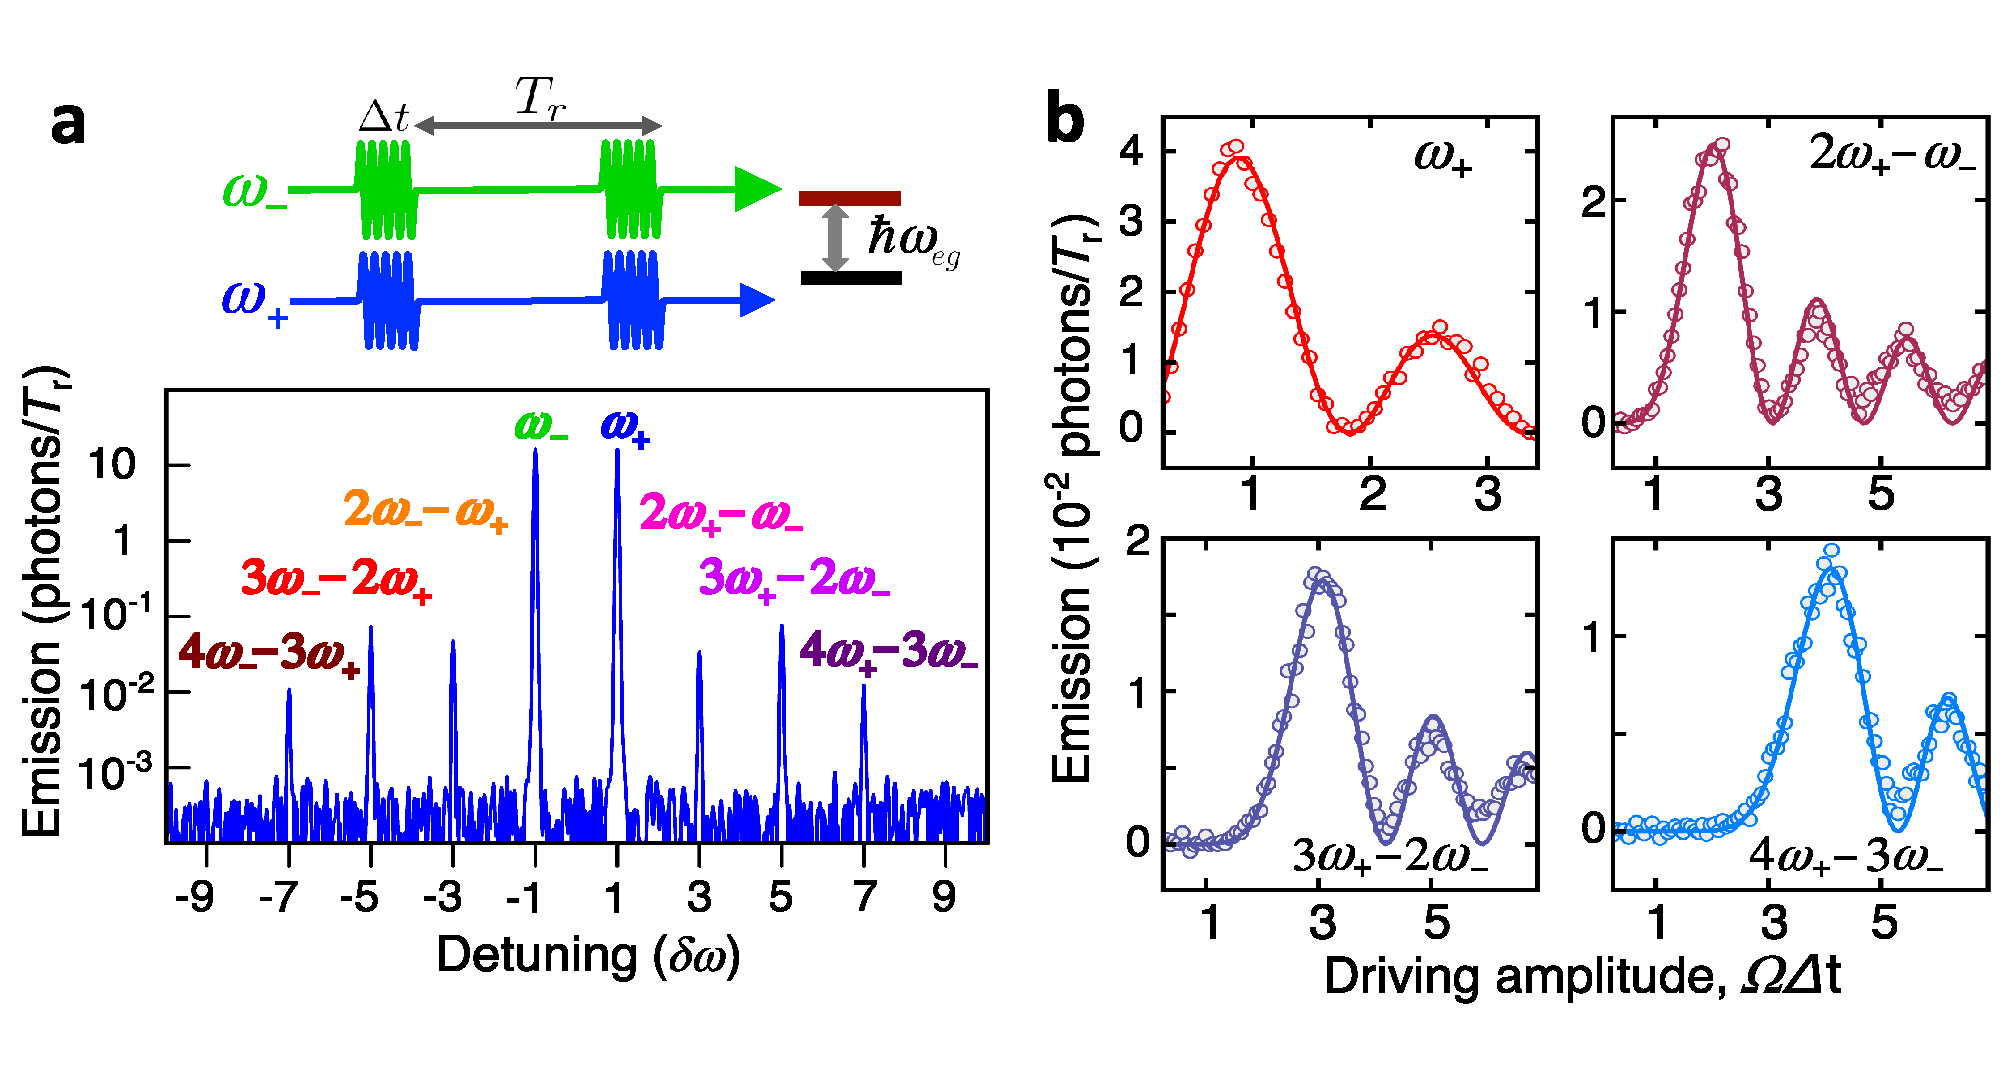
\includegraphics[width=1\textwidth]{Bessels.pdf}
\caption[Зависимость интенсивности боковых компонент от длительности импульсов $\Delta t$ бихроматической накачки]{Зависимость интенсивности боковых компонент от длительности импульсов $\Delta t$ бихроматической накачки}
\end{figure} 
\section{Введение задержки. Квантовое смешение волн}
\section{Квантовое смешение волн на 3-уровневой системе}
\section{Численный расчет импульсной динамики}
\section{Аналитический расчет в представлении вторичного квантования}

